\documentclass[a4paper, 12pt]{article}

\usepackage[T1]{fontenc}
\usepackage[utf8]{inputenc}
\usepackage[english]{babel}  % ngerman for German
\usepackage{lmodern}  % nicer font
\usepackage{geometry}
\geometry{%
	left   = 2.5cm,
	right  = 2.5cm,
	top    = 3cm,
	bottom = 3cm
}

\usepackage{textcomp}
\usepackage{gensymb}
\usepackage{amsmath,amssymb,amsfonts}
\usepackage{nicefrac}  % nicer inline fractions
\usepackage{tensor}  % allows fancy indices
\usepackage{siunitx}  % easy handling of value + unit (e.g. \SI{10}{\pF})
% \sisetup{}  % configure siunitx (e.g. locale = DE)
\sisetup{output-complex-root=\ensuremath{\mathrm{j}}, complex-root-position = before-number} % configures SI format 10 + j5 for complex numbers (instead of 10 + 5i)

\usepackage{listings}  % code listings
\usepackage{enumerate}
\usepackage{booktabs}  % nicer tables (e.g. \toprule)
\usepackage{verbatim}  % inline code (\verb||)
\usepackage{subcaption}  % captions for subplots
\usepackage[european, siunitx, RPvoltages]{circuitikz}  % draw circuit diagrams
\usepackage{enumitem}
\setlist[itemize]{label=\rule[0.5ex]{0.6ex}{0.6ex}} % black squares for itemize

\usepackage{pstool}  %% Tex fonts in EPS files
\usepackage{graphicx}
\graphicspath{{./figures/}}

\usepackage{etoolbox} % Needed for AtBeginEnvironment command (appendix handling)
\usepackage{appendix} % Appendices environment

\usepackage{csquotes} % removes biber warning
\usepackage[  % ieee style citations (e.g. [1])
	backend     = biber,
	maxbibnames = 99,
	autocite    = footnote,
	style	    = ieee,
	citestyle   = numeric-comp,
	doi=false, isbn=false
]{biblatex}
\addbibresource{bibliography/bibliography.bib}

\usepackage[nobiblatex]{xurl}  % line breaks in URLs
% last imports
\usepackage[bookmarksopen,colorlinks,citecolor=black,linkcolor=black, urlcolor = black]{hyperref}

% after hyperref! 
\usepackage[noabbrev, nameinlink]{cleveref} 
% e.g. \cref{label} or \Cref(label) for capital letter
% configure cleveref not to use brackets around equation references
\creflabelformat{equation}{#2\textup{#1}#3} % Equation references without parentheses
\AtBeginEnvironment{appendices}{\crefalias{section}{appendix}} % Appendix referencing (for cref "Appendix A" instead of "Section A")


% add missing hyphenations
\hyphenation{im-ple-men-ta-tions}

\title{ECS7012P - Music and Audio Programming\\
	   Assignment 2: Drum Machine}
\author{
  Max Tamussino, 200579179
}
\date{\today}


\begin{document}

\maketitle
\tableofcontents
\pagebreak

\section{Introduction} \label{sec:intro}
This report covers the implementation of a simple drum machine using the Bela Platform \cite{McPherson2015}. It features an accelerometer, the orientation of which is used to select one of five drum patterns. A drum pattern is a pre-defined pattern in which drum audio samples are played, such as the example depicted in \Cref{fig:drum-patterns}. Turning the sensor upside down plays the samples backwards. Additionally, a potentiometer is used to adjust the playing speed, while two buttons are used to calibrate the accelerometer, pause and unpause. Tapping the accelerometer will temporarily play a fill pattern and return to the pattern that played before after finishing.

\begin{figure}[h!]
	\centering
	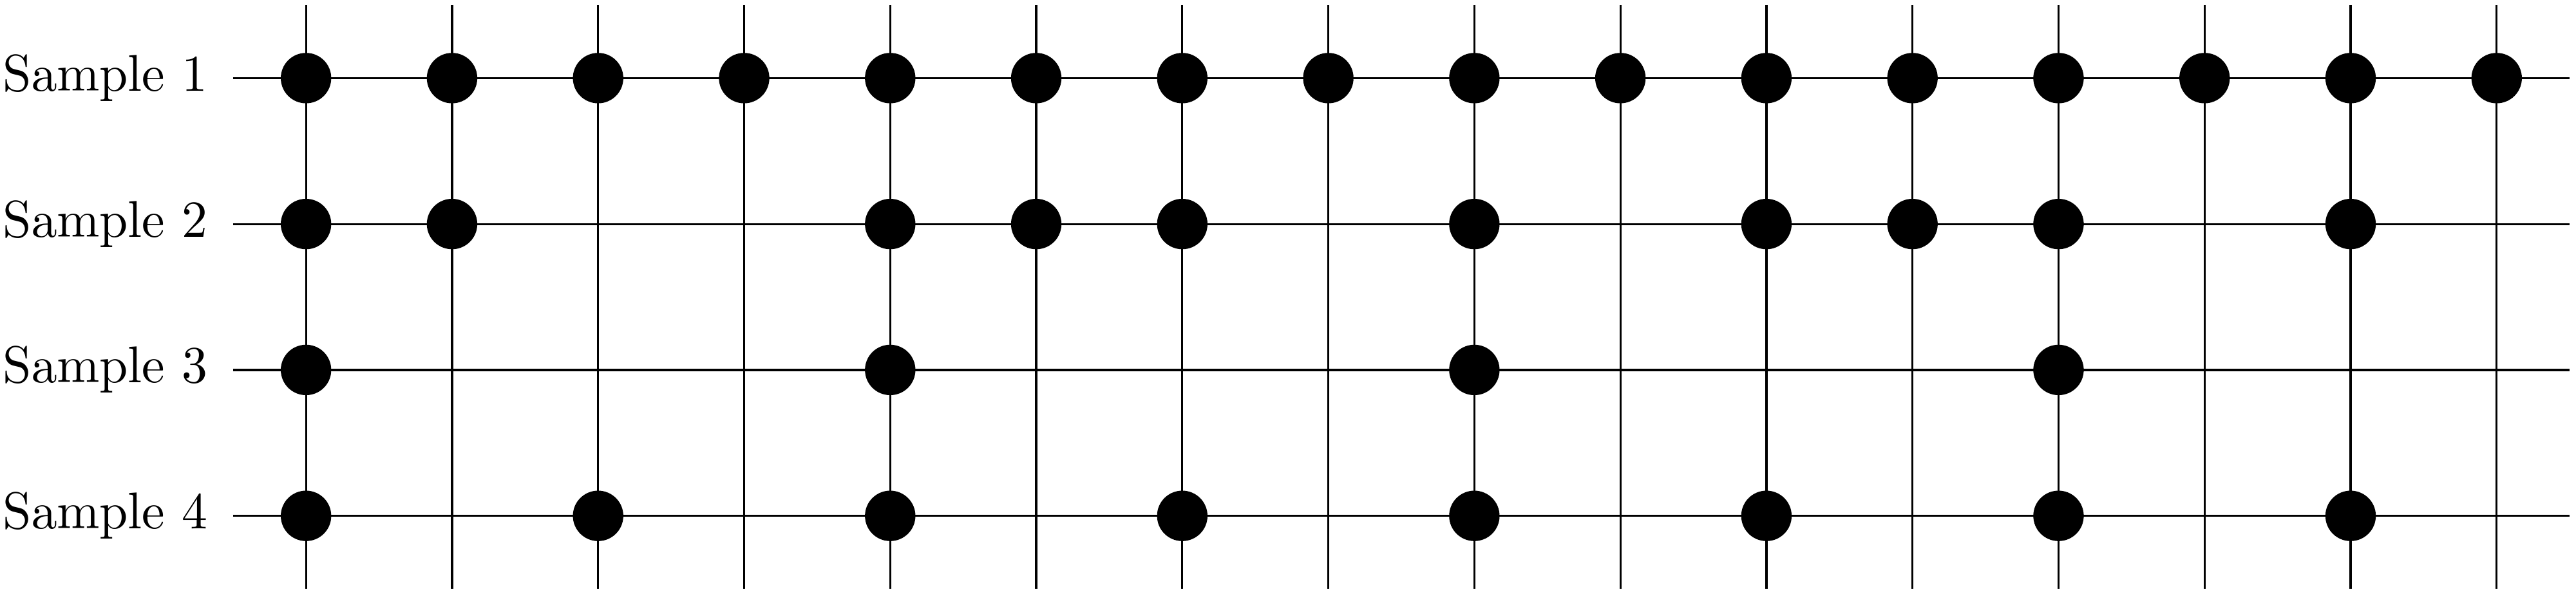
\includegraphics[width=\textwidth]{patterns.png}
	\caption{Example drum pattern consisting of four different audio samples}
	\label{fig:drum-patterns}
\end{figure}

\section{Accelerometer}
The accelerometer was mounted above the Bela board so that it could be moved into different orientations by hand, allowing control of the drum machine. The used sensor \emph{MMA7361} \cite{Freescale2008} has three analog outputs, each representing acceleration in one axis. Each of those channels shows a voltage $V_{off} \approx \SI{1.65}{\volt}$ when \SI{0}{\gram} is measured in its axis. In the selected measurement range of $\pm \SI{1.5}{\gram}$, the sensitivity is given by $S_{1.5g} \approx \SI{800}{\milli\volt\per\gram}$. These values were however discovered to be quite different for each channel, which is why it has to be calibrated upon powerup. 

\subsection{Calibration} \label{sec:calibration}
To obtain both $V_{off}$ and $S_{1.5g}$ for all three channels, the accelerometer has to be put into three positions. A button is used to signal that the accelerometer has been placed into one of these positions (the order does not matter). Each of them should measure \SI{+1}{\gram} in one and \SI{0}{\gram} in both other directions. The latter measurement directly yields $V_{0g} = V_{off}$ for its channels, while the measurement of $V_{1g}$ is used to calculate $S_{1.5g}$ by

\begin{equation}
	S_{1.5g} = \frac{V_{1g} - V_{0g}}{\SI{1}{\gram}}.
\end{equation}

After calibrating, the correct acceleration for each axis can be calculated by

\begin{equation}
	a = \frac{V_{in} - V_{off}}{S_{1.5g}}
\end{equation}

or (as it is implemented) directly by

\begin{equation}
	a = \frac{V_{in} - V_{0g}}{V_{1g} - V_{0g}} \cdot \SI{1}{\gram}.
\end{equation}

\subsection{Filters}
The output of the sensor was measured using the standard Bela analog sampling rate of \SI{22.05}{\kilo\hertz}. To reduce measurement noise and other influences like shaking of the controlling hand, this signal was filtered. A lowpass filter with a very low cutoff frequency is required to detect only changes in the steady-state orientation. At this high sampling rate a sufficiently low cutoff frequency is difficult to realise. FIR filters need to be of order $N>2000$ and IIR filters often become instable after transitioning to single-precision floating point calculations. This is why initially only a simple first-order IIR lowpass was used to remove measurement noise. The resulting smoother signal was sampled down by the factor $32$. This allowed the second stage lowpass filter to also consist of only one first-order IIR lowpass. The resulting signal was stable enough to be used to determine the current orientation state of the accelerometer. \Cref{fig:filtering} shows the $z$-axis acceleration transitioning from \SI{1}{\gram} to \SI{0}{\gram} in \SI{700}{\milli\second}. Both filters clearly show introduced latency.

\begin{figure}[h!]
	\centering
	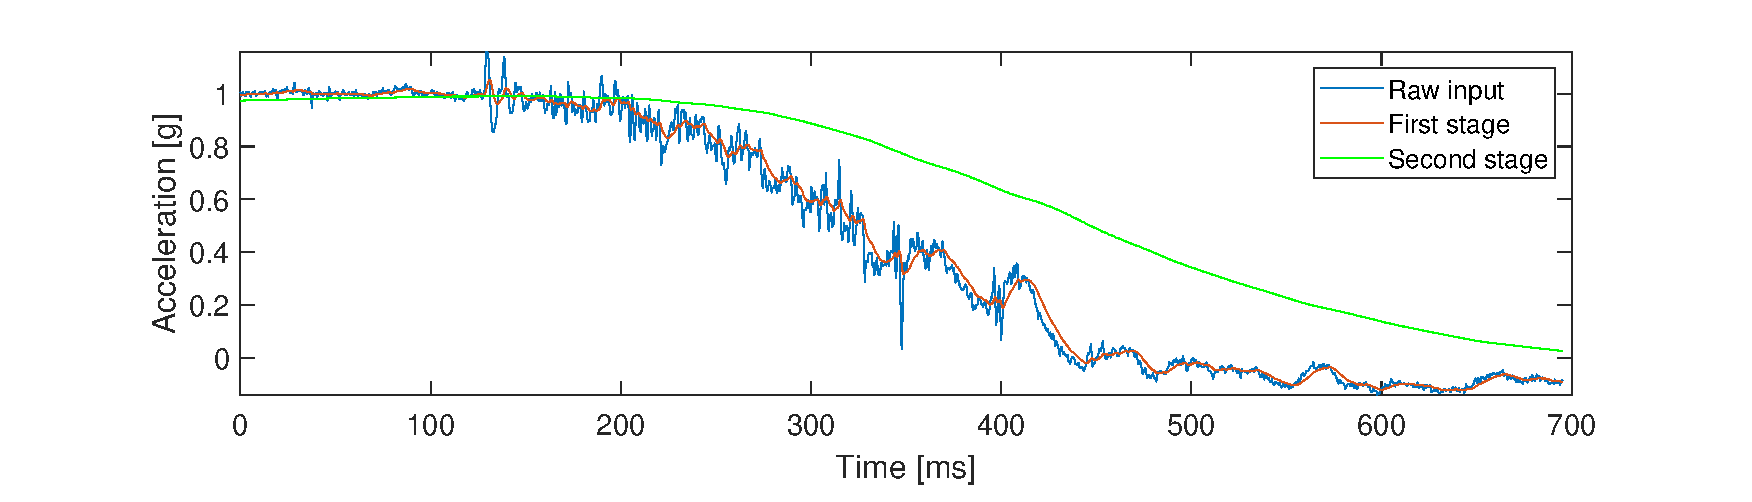
\includegraphics[width=\textwidth]{filters.eps}
	\caption{Result of the designed filter stages}
	\label{fig:filtering}
\end{figure}

\subsection{State machine}
Firstly, the measured acceleration values are examined for steadyness. If 

\begin{equation}
	|a| = \sqrt{a_x^2 + a_y^2 + a_z^2} > \SI{1.05}{\gram},
\end{equation}

the sample is considered unsteady and is discarded. This is because in this case additional acceleration components other than gravity are involved.

Otherwise, the current orientation of the calibrated accelerometer is determined using a state machine, which is depicted in \Cref{fig:stm}. Hysteresis was used to avoid bouncing between two states: A high threshold $t_{enter} = \SI{0.8}{\gram}$ and a low threshold $t_{exit} = \SI{0.6}{\gram}$ is defined. Starting in the intermediate state, it is checked whether any axis experiences acceleration by more than $t_{enter}$. If so, The according state is entered and only left again if the according acceleration falls below the lower $t_{exit}$.

\begin{figure}[h!]
	\centering
	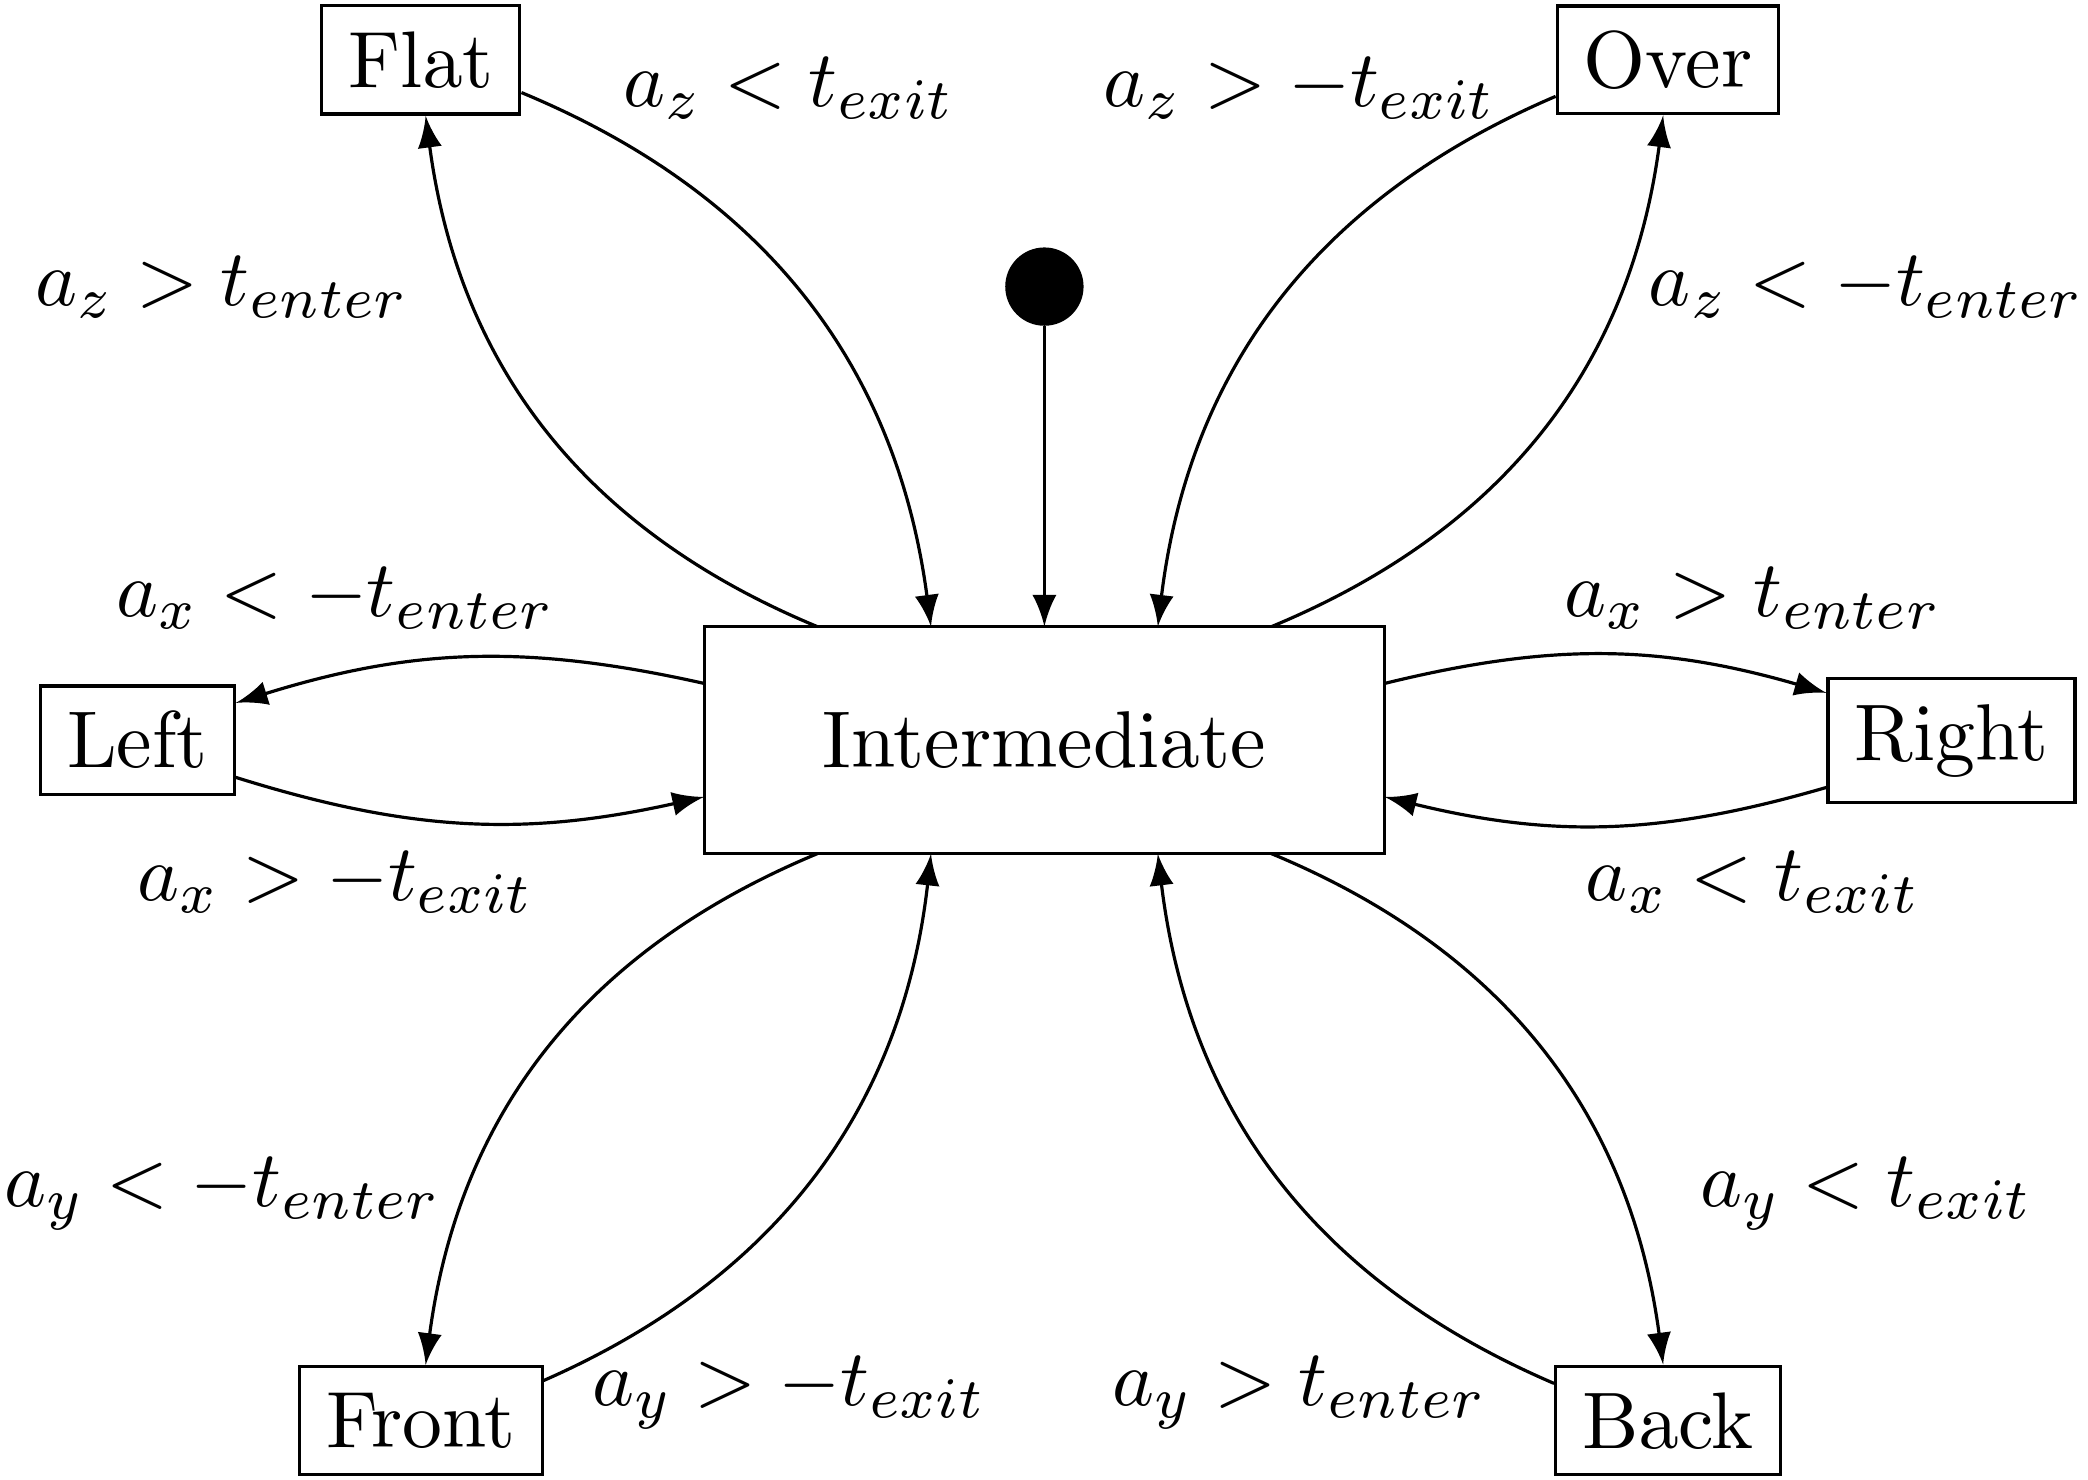
\includegraphics[width=0.65\textwidth]{stm.png}
	\caption{State machine to determine accelerometer orientation state}
	\label{fig:stm}
\end{figure}

Because the state machine enters a state before the theoretical maximum of \SI{1}{\gram}, this cancels the effect of the high latency introduced by the lowpass filters. This however depends strongly on the speed of the transition.

\subsection{Tap detection}
To detect a tap on the accelerometer, a high-pass filter may be implemented to only pass spikes in the acceleration. Alternatively, the total acceleration $|a|$ may be considered. Previously, the total acceleration was used to determine whether or not an acceleration sample is steady. For $|a| > \SI{1.05}{\gram}$, the sample is not considered for the calculation of the orientation. A simple higher threshold $|a| > \SI{1.1}{\gram}$ has however proven to be a reliable indicator for a tap on the accelerometer. This approach was considered superior to a high-pass filter as the value of $|a|$ was already calculated, the implementation is simpler and the tap can be detected from every direction.

\section{Other hardware}
A potentiometer is used to adjust the speed of the playing drum pattern. This does not affect the speed of individual samples, but the time between those. It may be adjusted to be bewteen \SIrange{50}{1000}{\milli\second}. Moreover, a LED lights up for \SI{2}{\milli\second} on each beat. One button makes the drum machine start and stop playing, another button is used to calibrate the accelerometer as described in \Cref{sec:calibration}.

\sloppy
\printbibliography

\end{document}